% --- Program Section ---

\newprogram{Program 3}{Implement findKthLargest(nums: List[int], k: int) -> int and findMinMax(nums:
List[int]) -> Tuple[int, int] functions accepting an unsorted array, returning the -th element
and min-max pair.}

\subsection*{Code}
\begin{lstlisting}[language=Python]
from typing import List, Tuple

def findKthLargest(nums: List[int], k: int) -> int:
    nums.sort(reverse=True)
    return nums[k - 1]


def findMinMax(nums: List[int]) -> Tuple[int, int]:
    return min(nums), max(nums)


# Example
nums = [3, 1, 5, 2, 4]

print("Kth largest:", findKthLargest(nums, 2))
print("Min and Max:", findMinMax(nums))

\end{lstlisting}

\subsection*{Output}
\begin{center}
    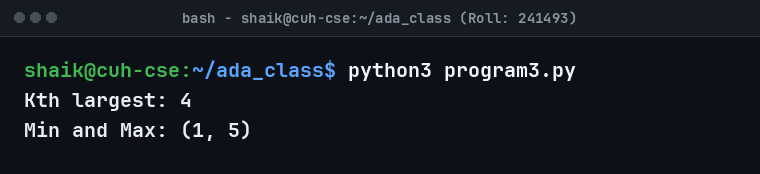
\includegraphics[width=0.88\textwidth]{Images/output_screenshot3.png}
\end{center}

\subsection*{GitHub Scan Code}
\begin{center}
    \begin{minipage}{0.3\textwidth}
        \centering
        % Generates a 2.5cm high QR code directly linking to the code file
        \qrcode[height=3.5cm]{https://github.com/gytdrop/ada_class/blob/main/program3.py} \\[0.2cm]
        \scriptsize\ttfamily Scan to view source code 
    \end{minipage}
\end{center}


% Add a horizontal line that indicates the END of the program.
\vspace{1cm}
\begin{center}
    \rule{1\textwidth}{1pt} % Clean, centered 1pt thick horizontal line
\end{center}